\begin{frame}
    \frametitle{Completed Stage II-2: ROLLO v1.0 Demonstration}
    \begin{itemize}
        \item I demonstrate ROLLO's capabilities with a single objective design 
        problem: maximize $k_{eff}$ by varying TRISO particle distribution in an 
        AHTR fuel slab while keeping total packing fraction constant
        \item I divided the slab into ten cells along the x-axis between the FliBe and 
        graphite buffers, resulting in ten cells. A sine distribution governs the 
        TRISO particle packing fraction's distribution across cells:
    \end{itemize}
    \small
    \begin{align*}
        PF(x) &= \left(a\cdot sin(b\cdot x + c) + 2\right) \cdot NF\\
        \intertext{where}
        PF &= \mbox{packing fraction } [-] \nonumber \\ 
        a &= \mbox{amplitude, peak deviation of the function from zero } [-] \nonumber \\
        b &= \mbox{angular frequency, rate of change of the function argument } [\frac{radians}{cm}] \nonumber \\
        c &= \mbox{phase, the position in its cycle the oscillation is at t = 0 } [radians]\nonumber \\
        x &= \mbox{midpoint value for each cell } [cm]\nonumber \\
        NF &= \mbox{Normalization factor } [-]\nonumber
    \end{align*}
\end{frame}

\begin{frame}
    \frametitle{Completed Stage II-2: Prolem Defintion}
    \begin{figure}[]
        \centering
        \makebox[\textwidth][c]{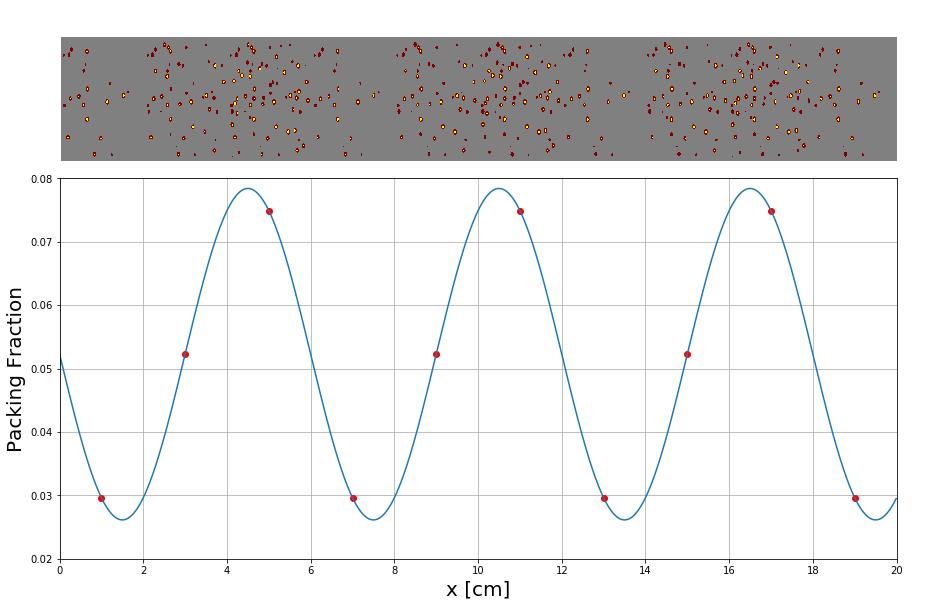
\includegraphics[width=0.9\linewidth]{../docs/figures/triso_distribution_sine.png}} 
        \caption{Above: Straightened AHTR fuel slab with varying TRISO particle 
        distribution across ten cells based on the sine distribution. 
        Below: $PF(x) = (0.5\ sin(\frac{\pi}{3}x + \pi) + 2)  \times NF$ 
        sine distribution with red points indicating the packing fraction at each cell. }
    \end{figure}
\end{frame}

\begin{frame}
    \frametitle{Completed Stage II-2: Hyperparameter Search}
    \begin{itemize}
        \item In a ROLLO input file, the user defines hyperparameters for the genetic 
        algorithm. A good hyperparameter set guides the optimization process by 
        balancing exploitation and exploration to find an optimal solution quickly 
        and accurately. 
        \item I performed the hyperparameter search with a coarse-to-fine random sampling scheme
        \item The hyperparameters varied included population size, number of generations, 
        mutation probability, mating probability, selection operator, selection operator's 
        number of individuals, selection operator's tournament size, mutation operator, 
        and mating operator.  
        \item I started with 25 coarse experiments and fine-tuned the hyperparameters
        with 15 more experiments. For each genetic algorithm experiment, the number 
        of OpenMC evaluations remained constant at 600
    \end{itemize}
\end{frame}

\begin{frame}
    \frametitle{Completed Stage II-2: Hyperparameter Search}
    \begin{figure}
        \caption{Hyperparameter search is conducted in three phases: \textit{Coarse Search}, 
    \textit{Fine Search 1}, \textit{Fine Search 2}. Each hyperparameter's lower and
    upper bounds for each search phase are listed.}
        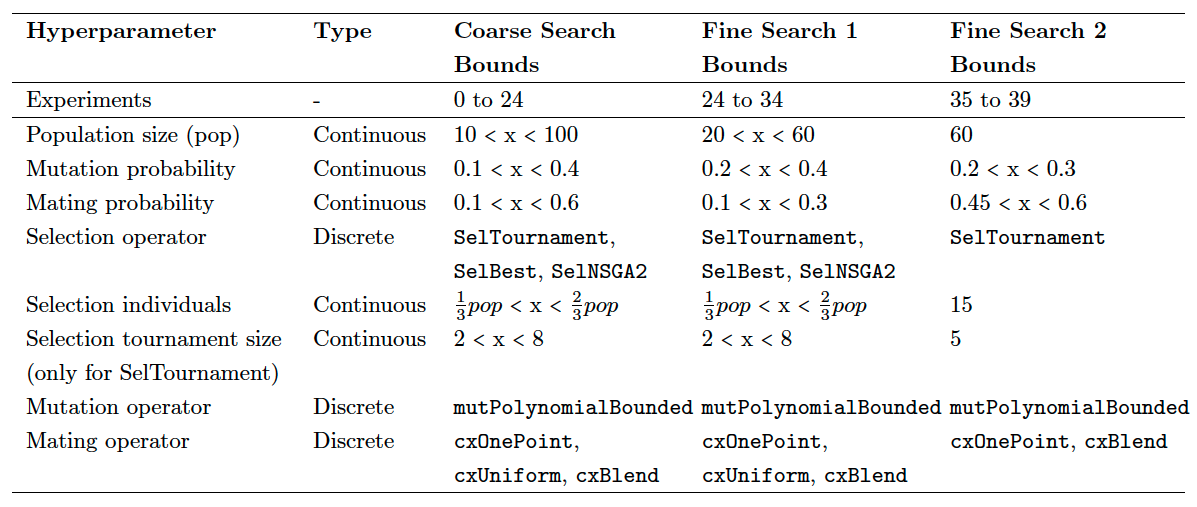
\includegraphics[width=0.8\linewidth]{figures/hyperparameter-search.png} 
    \end{figure}
\end{frame}

\begin{frame}
    \frametitle{Completed Stage II-2: Hyperparameter Search}
    \begin{figure}[]
        \centering
        \makebox[\textwidth][c]{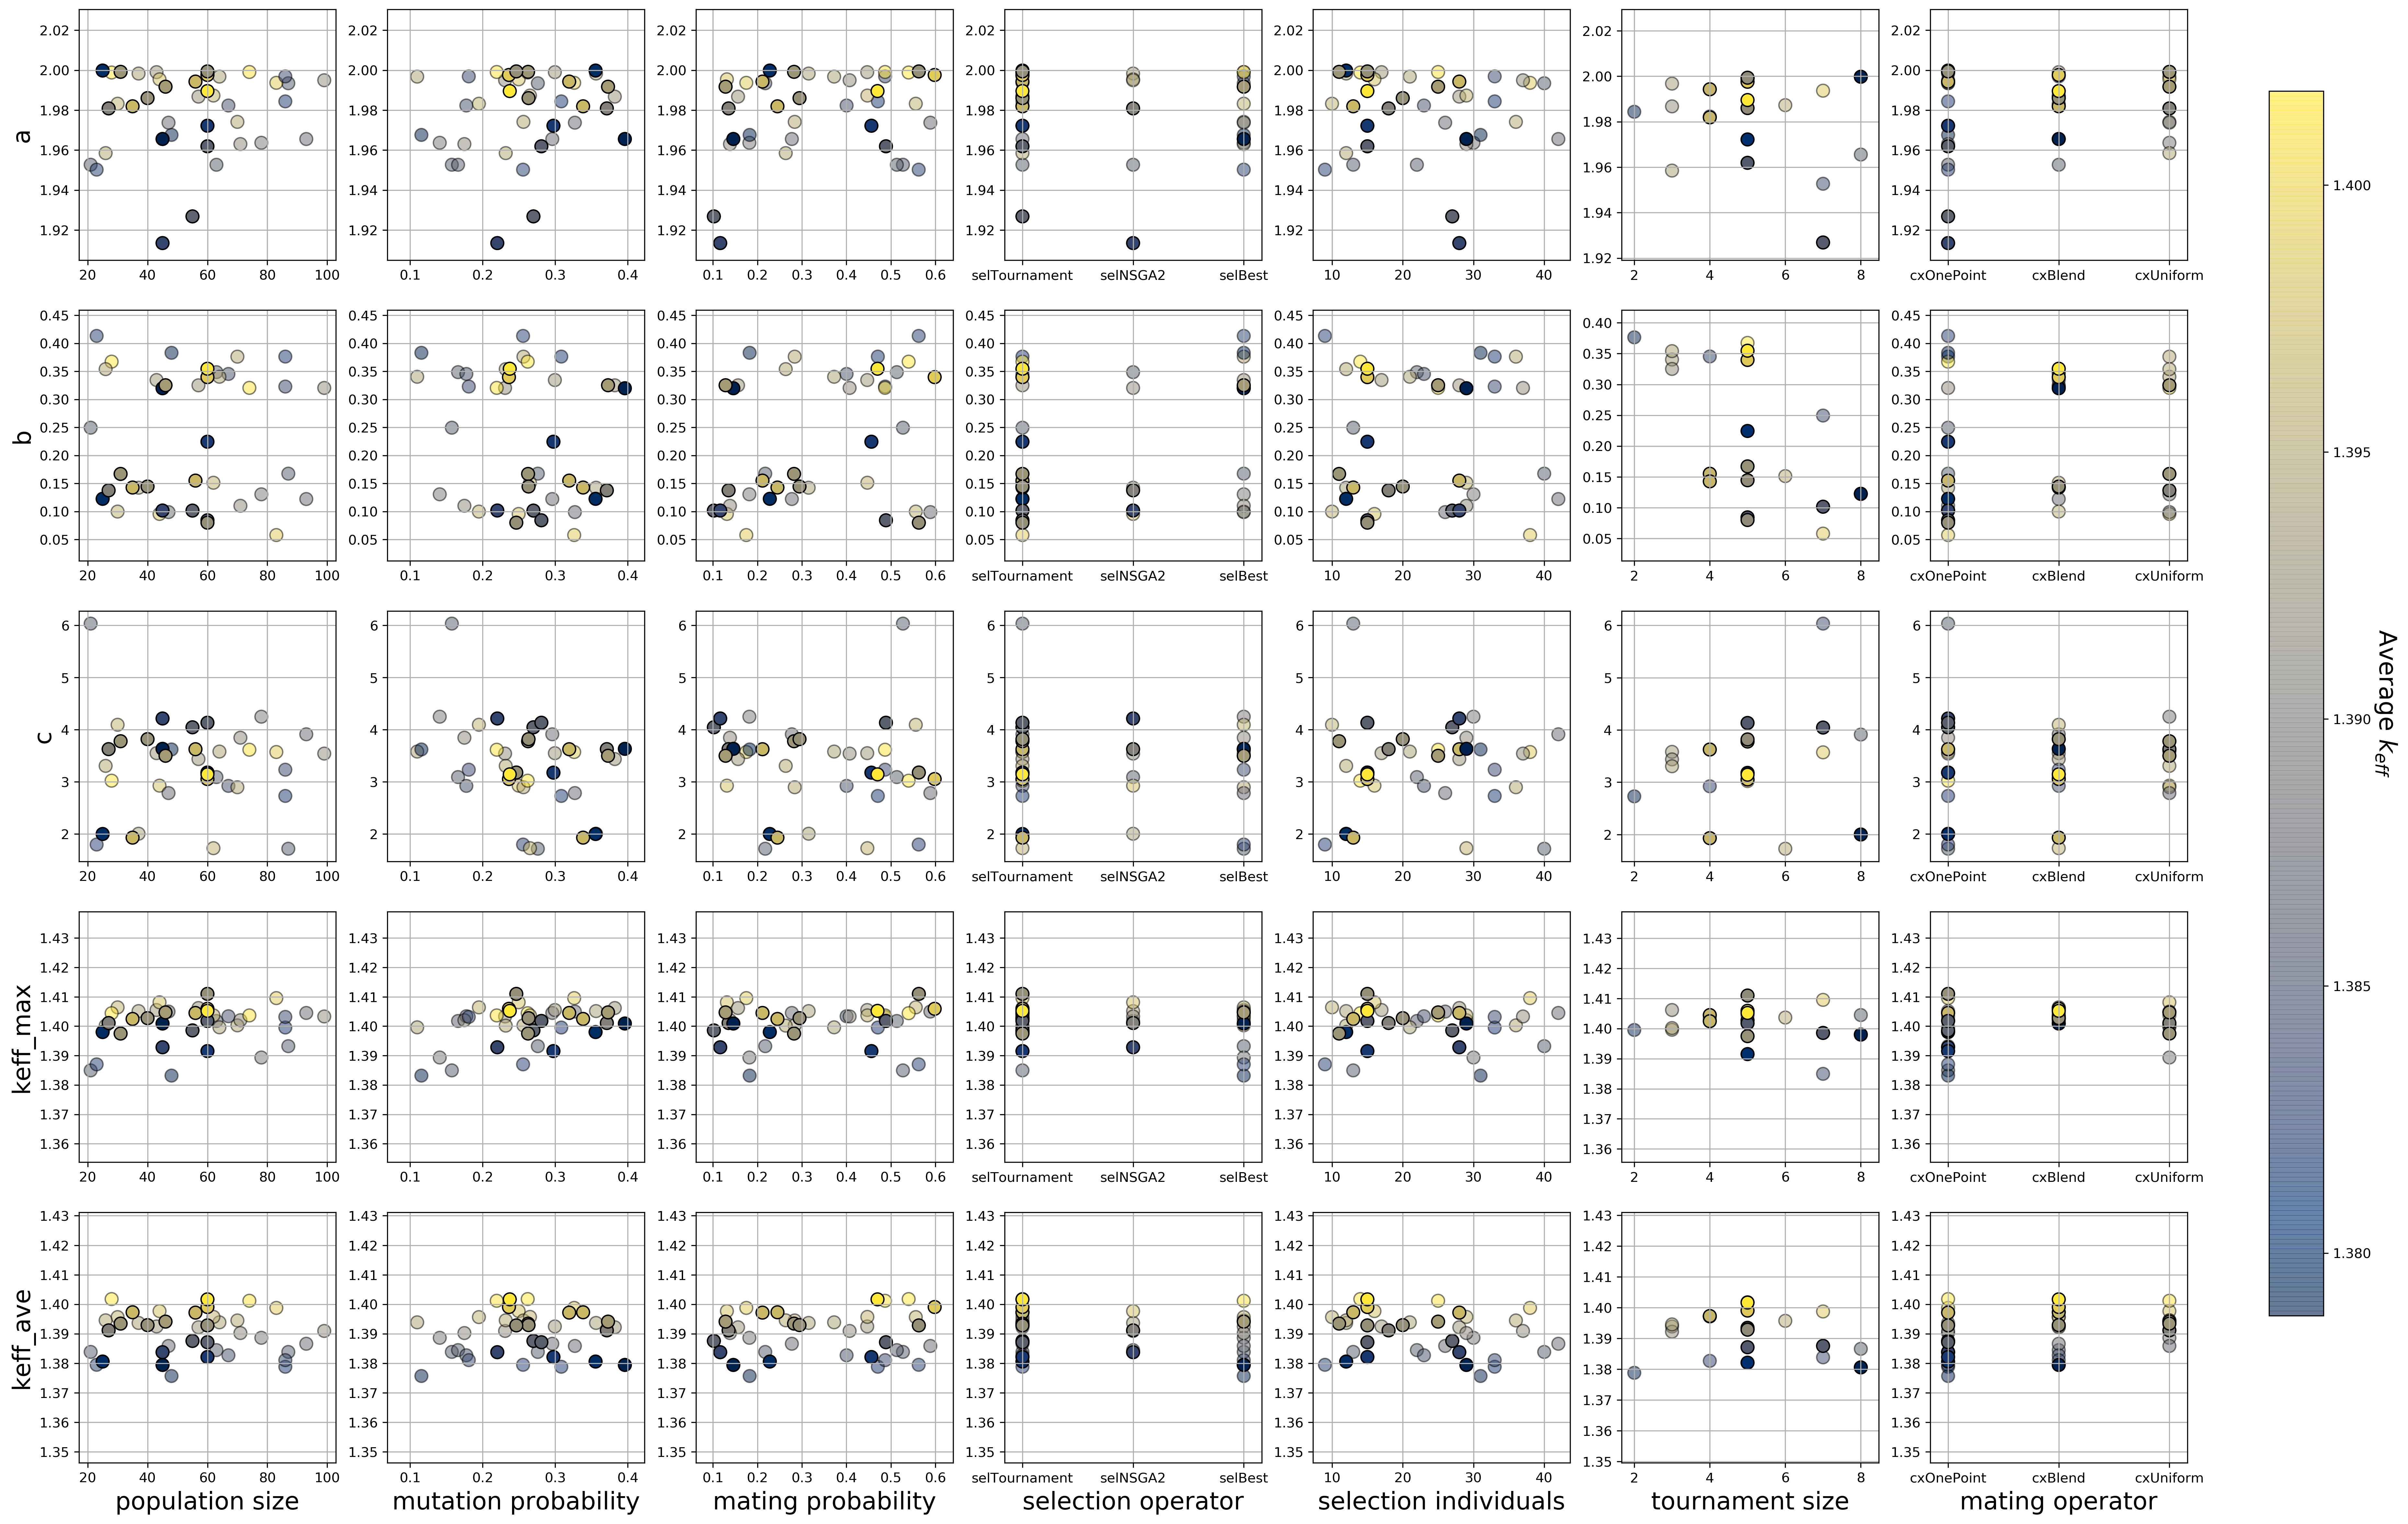
\includegraphics[width=0.65\linewidth]{../docs/figures/input_hyperparameters_sens.png}} 
        \caption{Hyperparameters search's results for all 40 experiments (coarse 
        and fine). I plotted the hyperparameters against: a,b,c control parameters, 
        each experiment's final generation $k_{eff max}$, and final generation 
        $\overline{k_{eff}}$ with a third color dimension representing each experiment's final 
        population's $\overline{k_{eff}}$ (color bar representing the $k_{eff}$ values 
        provided on the right side of the figure). Coarse experiments' (0 to 24) scatter points 
        are $50\%$ transparent, while the fine experiments' (24 to 39) scatter points 
        are opaque.}
    \end{figure}
\end{frame}

\begin{frame}
    \frametitle{Completed Stage II-2: Results from best hyperparameter set}
    \begin{itemize}
        \item I define the best-performing hyperparameter set as the experiment that produces 
        the highest $\overline{k_{eff}}$ in its final generation. 
    \end{itemize}
    \begin{figure}[]
        \centering
        \makebox[\textwidth][c]{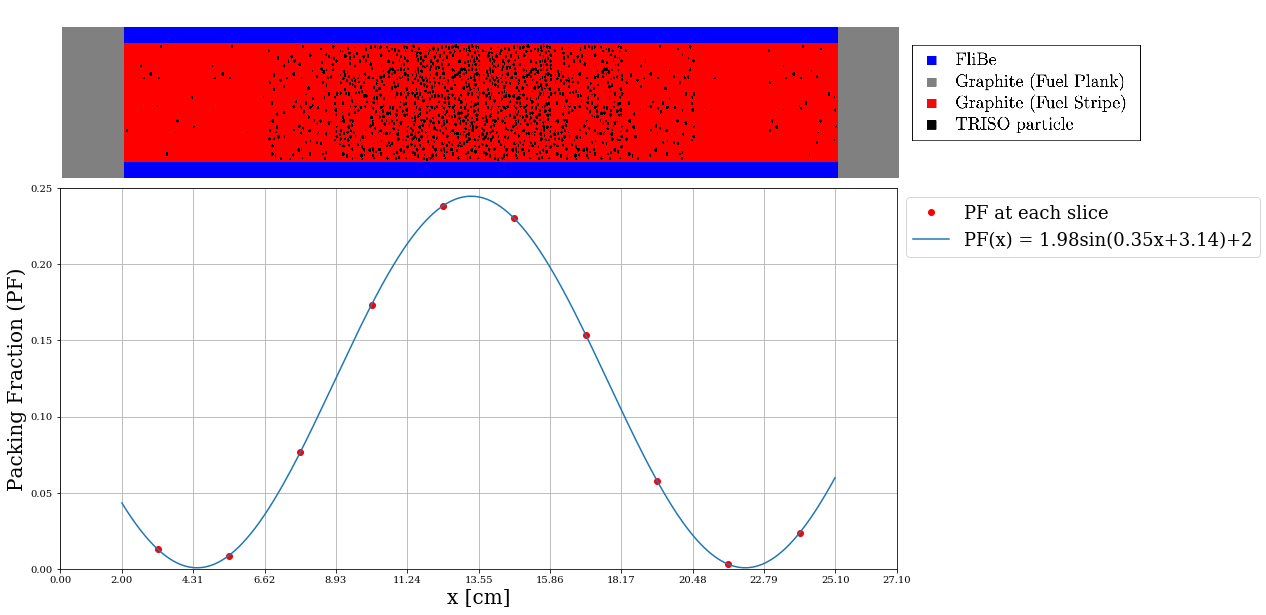
\includegraphics[width=0.75\linewidth]{../docs/figures/triso_distribution_sine_39.png}} 
        \caption{Experiment 39 packing distribution that produced $k_{eff max} = 1.40519 \pm 0.00130$. 
        Below: $PF(x) = (1.98\ sin(0.35x+3.14)+2)  \times NF$ sine distribution with 
        red points indicating the packing fraction at each cell. 
        Above: Straightened AHTR fuel slab with varying TRISO particle 
        distribution across ten cells based on the sine distribution. }
        \label{fig:triso_distribution_sine_39}
    \end{figure}
    
\end{frame}